\documentclass[12pt,reqno]{amsart}
%\documentclass[../Solutions_Introduction_to_Algorithms.tex]{subfiles}
\usepackage{amsmath,amsfonts,amscd,amssymb,epsf,color,enumerate,graphicx,url}
\usepackage{algorithm, algorithmic}
\usepackage{forest, tikz, xcolor}
\usetikzlibrary{matrix, positioning}
\setlength{\oddsidemargin}{-0.2in}%
\setlength{\evensidemargin}{-0.2in}%
\setlength{\textwidth}{6.6in}%
\setlength{\topmargin}{-0.5in}%
 \setlength{\textheight}{9.5in}%
 \definecolor{orange}{rgb}{1,0.5,0}
 \pagestyle{plain}
\linespread{1.3}
\usepackage[small]{caption}
\newcommand{\pa}{\partial}
\newcommand{\va}{\vspace{0.4cm}}
\newcommand{\di}{\displaystyle}
\newcommand{\disp}{\displaystyle}


% turn on \answertrue to show the solution
% turn on \answerfalse to hide the solution
\newif\ifanswer
\answertrue
%\answerfalse



\begin{document}
\noindent {\footnotesize Introduction to Algorithms}\hspace{10.5cm} {\footnotesize Solutions}

\vspace{0.5cm}
\hspace{5.5cm}\textbf{\large Problems in Chapter 7}
\vspace{0.5cm}

\begin{enumerate}[1.]

\item \textbf{Hoare partition correctness}\\ The version of $\textsc{Partition}$ given in this chapter is not the original partitioning algorithm. Here is the original partitioning algorithm, which is due to C.A.R. Hoare.
\begin{algorithm}
    \caption{$\textsc{Hoare-Partition}(A, p, r)$}
    \begin{algorithmic}[1]
        \STATE $x = A[p]$
        \STATE $i = p - 1$
        \STATE $j = r + 1$
        \WHILE{\textbf{True}}
            \REPEAT
                \STATE $j = j - 1$
            \UNTIL{$A[j] \leq x$}
            \REPEAT
                \STATE $i = i + 1$
            \UNTIL{$A[i] \geq x$}
            \IF{$i < j$}
                \STATE exchange $A[i]$ with $A[j]$
            \ELSE
                \RETURN $j$
            \ENDIF
        \ENDWHILE
    \end{algorithmic}
\end{algorithm}
\begin{enumerate}
    \item[a.] Demonstrate the operation of $\textsc{Hoare-Partition}$ on the array $A = \langle 13, 19, 9, 5, 12, 8, 7,$ $4, 11, 2, 6, 21 \rangle$, showing the values of the array and the indices $i$ and $j$ after each iteration of the \textbf{while} loop in lines 4-13.
    \ifanswer
    \noindent {\bf \\Solution}
    In the \textbf{while} loop in lines 4-13, the program looks for the rightmost element that is smaller than or equal to $x$, and the leftmost element that is greater than or equal to $x$, and swap them if they are not the same element. With this procedure, the entries that $i$ passes by are all smaller than $x$, and the entries that $j$ passes by are all greater than $x$.\\
    In this example, $x = A[p] = 13$. Below shows the procedure of $\textsc{Hoare-Partition}$ in sorting the array $A$:
    \newpage
    \begin{center}
        \begin{tikzpicture}
            \matrix[matrix of nodes,
                    nodes={draw, minimum width=1cm, minimum height=1cm, anchor=center},
                    column sep=0pt, row sep=0pt,
                    name=m1] 
            {
                \node[fill=none, draw=none, name=m1-0] {~}; &
                \node[fill=lightgray, name=m1-1] {13}; &
                \node[fill=lightgray, name=m1-2] {19}; &
                \node[fill=lightgray, name=m1-3] {9}; &
                \node[fill=lightgray, name=m1-4] {5}; &
                \node[fill=lightgray, name=m1-5] {12}; &
                \node[fill=lightgray, name=m1-6] {8}; &
                \node[fill=lightgray, name=m1-7] {7}; &
                \node[fill=lightgray, name=m1-8] {4}; &
                \node[fill=lightgray, name=m1-9] {11}; &
                \node[fill=lightgray, name=m1-10] {2}; &
                \node[fill=lightgray, name=m1-11] {6}; &
                \node[fill=lightgray, name=m1-12] {21}; &
                \node[fill=none, draw=none, name=m1-13] {~}; \\
            };
            \node[above=2pt of m1-0] {\textit{i}};
            \node[above=2pt of m1-1] {\textit{p}};
            \node[above=2pt of m1-12] {\textit{r}};
            \node[above=2pt of m1-13] {\textit{j}};

            \matrix[matrix of nodes,
                    nodes={draw, minimum width=1cm, minimum height=1cm, anchor=center},
                    column sep=0pt, row sep=0pt,
                    below=1cm of m1,
                    name=m2] 
            {
                \node[fill=none, draw=none, name=m2-0] {~}; &
                \node[fill=pink, name=m2-1] {6}; &
                \node[fill=lightgray, name=m2-2] {19}; &
                \node[fill=lightgray, name=m2-3] {9}; &
                \node[fill=lightgray, name=m2-4] {5}; &
                \node[fill=lightgray, name=m2-5] {12}; &
                \node[fill=lightgray, name=m2-6] {8}; &
                \node[fill=lightgray, name=m2-7] {7}; &
                \node[fill=lightgray, name=m2-8] {4}; &
                \node[fill=lightgray, name=m2-9] {11}; &
                \node[fill=lightgray, name=m2-10] {2}; &
                \node[fill=cyan, name=m2-11] {13}; &
                \node[fill=cyan, name=m2-12] {21}; &
                \node[fill=none, draw=none, name=m2-13] {~}; \\
            };
            \node[above=2pt of m2-1] {\textit{p, i}};
            \node[above=2pt of m2-11] {\textit{j}};
            \node[above=2pt of m2-12] {\textit{r}};

            \matrix[matrix of nodes,
                    nodes={draw, minimum width=1cm, minimum height=1cm, anchor=center},
                    column sep=0pt, row sep=0pt,
                    below=1cm of m2,
                    name=m3] 
            {
                \node[fill=none, draw=none, name=m3-0] {~}; &
                \node[fill=pink, name=m3-1] {6}; &
                \node[fill=pink, name=m3-2] {2}; &
                \node[fill=lightgray, name=m3-3] {9}; &
                \node[fill=lightgray, name=m3-4] {5}; &
                \node[fill=lightgray, name=m3-5] {12}; &
                \node[fill=lightgray, name=m3-6] {8}; &
                \node[fill=lightgray, name=m3-7] {7}; &
                \node[fill=lightgray, name=m3-8] {4}; &
                \node[fill=lightgray, name=m3-9] {11}; &
                \node[fill=cyan, name=m3-10] {19}; &
                \node[fill=cyan, name=m3-11] {13}; &
                \node[fill=cyan, name=m3-12] {21}; &
                \node[fill=none, draw=none, name=m2-13] {~}; \\
            };
            \node[above=2pt of m3-1] {\textit{p}};
            \node[above=2pt of m3-2] {\textit{i}};
            \node[above=2pt of m3-10] {\textit{j}};
            \node[above=2pt of m3-12] {\textit{r}};

            \matrix[matrix of nodes,
                    nodes={draw, minimum width=1cm, minimum height=1cm, anchor=center},
                    column sep=0pt, row sep=0pt,
                    below=1cm of m3,
                    name=m4] 
            {
                \node[fill=none, draw=none, name=m3-0] {~}; &
                \node[fill=pink, name=m4-1] {6}; &
                \node[fill=pink, name=m4-2] {2}; &
                \node[fill=pink, name=m4-3] {9}; &
                \node[fill=pink, name=m4-4] {5}; &
                \node[fill=pink, name=m4-5] {12}; &
                \node[fill=pink, name=m4-6] {8}; &
                \node[fill=pink, name=m4-7] {7}; &
                \node[fill=pink, name=m4-8] {4}; &
                \node[fill=yellow, name=m4-9] {11}; &
                \node[fill=cyan, name=m4-10] {19}; &
                \node[fill=cyan, name=m4-11] {13}; &
                \node[fill=cyan, name=m4-12] {21}; &
                \node[fill=none, draw=none, name=m2-13] {~}; \\
            };
            \node[above=2pt of m4-1] {\textit{p}};
            \node[above=2pt of m4-9] {\textit{j}};
            \node[above=2pt of m4-10] {\textit{i}};
            \node[above=2pt of m4-12] {\textit{r}};
        \end{tikzpicture}
    \end{center}
    Finally, $j = 9$ is returned, and the array $A$ is separated into two subarrays $\langle 6, 2, 9, 5, 12,$ $8, 7, 4\rangle$ and $\langle 19, 13, 21 \rangle$.

    \item[b.] Describe how the $\textsc{Partition}$ procedure in Section 7.1 differs from $\textsc{Hoare-Partition}$ when all elements in $A[p: r]$ are equal. Describe a practical advantage of $\textsc{Hoare}$-$\textsc{Partition}$ over $\textsc{Partition}$ for use in quicksort.
    \ifanswer
    \noindent {\bf \\Solution}
    In Exercise 7.1-2, we have shown that if all elements in the subarray $A[p: r]$ are equal, the program $\textsc{Partition}(A, p, r)$ returns $r$. In $\textsc{Hoare-Partition}(A, p, r)$, however, if all elements are equal, the program will swap the first and the last element, swap the second and last second element, \dots, until $i$ and $j$ meet. The final value of $j$, which is returned, is almost the middle of $A[p, r]$ (in fact, it is $\lfloor (p + r)/2 \rfloor$).\\
    In practice, especially when there are repeated values in the array, $\textsc{Hoare-Partition}$ tends to divide the subarray in a more balanced way, reducing the average running time.
\end{enumerate}
The next three questions ask you to give a careful argument that the procedure $\textsc{Hoare}$-$\textsc{Partition}$ is correct. Assuming that the subarray $A[p: r]$ contains at least two elements, prove the following:

\begin{enumerate}
    \item[c.] The indices $i$ and $j$ are such that the procedure never accesses an element of $A$ outside the subarray $A[p: r]$.
    \ifanswer
    \noindent {\bf \\Solution}
    In the first iteration, since $x = A[p]$, the final value of $i$ is $p$, and the final value of $j$ is at least $p$ and at most $r$. Now, suppose at the end of an iteration we have $p \leq i \leq r$ and $p \leq j \leq r$. If the loop is not terminated and we proceed to the next iteration, it is easy to see that $i < j$ and $A[i] \leq A[j]$. With these relations, in the next iteration, the new position of $i$ is at most the old position of $j$, and the new position of $j$ is at least the old position of $i$, again yielding $p \leq i \leq r$ and $p \leq j \leq r$. \qed
    
    \item[d.] When $\textsc{Hoare-Partition}$ terminates, it returns a value $j$ such that $p \leq j < r$.
    \ifanswer
    \noindent {\bf \\Solution}
    It suffices to show $j \neq r$. If the \textbf{for} loop terminates in the first iteration, then $j = i = p \neq r$. Otherwise, there are at least $2$ iterations, and $j$ decreases by at least $2$, that is, the final value of $j$ is less than or equal to $(r + 1) - 2 = r - 1 < r$. \qed
    
    \item[e.] Every element of $A[p: j]$ is less than or equal to every element of $A[j + 1: r]$ when $\textsc{Hoare-Partition}$ terminates.
    \ifanswer
    \noindent {\bf \\Solution}
    As discussed in a., all elements in $A[p: i - 1]$ are smaller than or equal to $x$, and all elements in $A[j + 1: r]$ are greater than or equal to $x$. When $\textsc{Hoare-Partition}$ terminates, we have $i \geq j$. The proof is almost done except possibly $i = j$ and we need to show $A[j] \leq x$. This is also obvious because $i = j$ implies $A[i] = A[j] = x$. \qed
\end{enumerate}
The $\textsc{Partition}$ procedure in Section 7.1 separates the pivot value (originally in $A[r$]) from the two partitions it forms. The $\textsc{Hoare-Partition}$ procedure, on the other hand, always places the pivot value (originally in $A[p]$) into one of the two partitions $A[p: j]$ and $A[j + 1: r]$. Since $p \leq j < r$, neither partition is empty.
\begin{enumerate}
    \item[f.] Rewrite the $\textsc{Quicksort}$ procedure to use $\textsc{Hoare-Partition}$.
    \ifanswer
    \noindent {\bf \\Solution}
    \begin{algorithm}
        \caption{$\textsc{Quicksort}(A, p, r)$}
        \begin{algorithmic}[1]
            \IF{$p \neq r$}
                \STATE $q = \textsc{Hoare-Partition}(A, p, r)$
                \STATE $\textsc{Quicksort}(A, p, q)$
                \STATE $\textsc{Quicksort}(A, q + 1, r)$
            \ENDIF
        \end{algorithmic}
    \end{algorithm}
\end{enumerate}
\vspace{1cm}



\item \textbf{Quicksort with equal element values}\\ The analysis of the expected running time of randomized quicksort in Section 7.4.2 assumes that all element values are distinct. This problem examines what happens when they are not.
\begin{enumerate}
    \item[a.] Suppose that all element values are equal. What is randomized quicksort's running time in this case?
    \ifanswer
    \noindent {\bf \\Solution}
    Since all elements in the array are equal, the randomized array has no difference. The associated recurrence is
    $$
    T(n) = T(n - 1) + \Theta(n)
    $$
    with solution $T(n) = \Theta(n^2)$.

    \item[b.] The $\textsc{Partition}$ procedure returns an index $1$ such that each element of $A[p: q - 1]$ is less than or equal to $A[q]$ and each element of $A[q + 1: r]$ is greater than $A[q]$. Modify the $\textsc{Partition}$ procedure to produce a procedure $\textsc{Partition'}(A, p, r)$, which permutes the elements of $A[q: r]$ and returns two indices $q$ and $t$, where $p \leq q \leq t \leq r$, such that
    \begin{itemize}
        \item all elements of $A[q: t]$ are equal,
        \item each element of $A[p: q - 1]$ is less than $A[q]$, and
        \item each element of $A[t + 1: r]$ is greater than $A[q]$.
    \end{itemize}
    Like $\textsc{Partition}$, your $\textsc{Partition'}(A, p, r)$ procedure should take $\Theta(r - p)$ time.
    \ifanswer
    \noindent {\bf \\Solution}
    \begin{algorithm}
        \caption{$\textsc{Partition'}(A, p, r)$}
        \begin{algorithmic}[1]
            \STATE $x = A[r]$
            \STATE $i = p - 1$
            \FOR{$j = p$ to $r - 1$}
                \IF{$A[j] \leq x$}
                    \STATE $i = i + 1$
                    \STATE exchange $A[i]$ with $A[j]$
                \ENDIF
            \ENDFOR
            \STATE exchange $A[i + 1]$ with $A[r]$
            \STATE $t = i + 1$
            \WHILE{$i \geq p$ and $A[i] == A[t]$}
                \STATE $i = i - 1$
            \ENDWHILE
            \STATE $k = p$
            \WHILE{$k < i$}
                \IF{$A[k] == A[t]$}
                    \STATE exchange $A[k]$ with $A[i]$
                    \WHILE{$i \geq p$ and $A[i] == A[t]$}
                        \STATE $i = i - 1$
                    \ENDWHILE
                \ENDIF
                \STATE $k = k + 1$
            \ENDWHILE
            \RETURN $i + 1, t$
        \end{algorithmic}
    \end{algorithm}
    \\Let $n = r - p + 1$ be the size of the subarray, and note that $\Theta(n) = \Theta(r - p)$. In each of the \textbf{while} loop starting at line 15, $k$ decreases by $1$, so there are $O(n)$ iterations in total. The \textbf{while} loop starting at line 18 looks terrible, but since $i$ decreases by $1$ in each iteration, the total number of iterations of this nested \textbf{while} loop over the whole program is $O(n)$. Hence, the running time of $\textsc{Partition'}(A, p, r)$ is $O(n)$.
    
    \item[c.] Modify the $\textsc{Randomized-Partition}$ procedure to call $\textsc{Partition'}$, and name the new procedure $\textsc{Randomized-Partition'}$. Then modify the $\textsc{Quicksort}$ procedure to produce a procedure $\textsc{Quicksort'}(A, p, r)$ that calls $\textsc{Randomized-Partition'}$ and recurses only on partitions where elements are not known to be equal to each other.
    \ifanswer
    \noindent {\bf \\Solution}
    \begin{algorithm}
        \caption{$\textsc{Randomized-Partition'}(A, p, r)$}
        \begin{algorithmic}[1]
            \STATE $i = \textsc{Random}(p, r)$
            \STATE exchange $A[p]$ with $A[i]$
            \RETURN $\textsc{Partition'}(A, p, r)$
        \end{algorithmic}
    \end{algorithm}
    \begin{algorithm}
        \caption{$\textsc{Quicksort'}(A, p, r)$}
        \begin{algorithmic}[1]
            \IF{$p < r$}
                \STATE $q, t = \textsc{Randomized-Partition'}(A, p, r)$
                \STATE $\textsc{Quicksort'}(A, p, q - 1)$
                \STATE $\textsc{Quicksort'}(A, t + 1, r)$
            \ENDIF
        \end{algorithmic}
    \end{algorithm}
    
    \item[d.] Using $\textsc{Quicksort'}$, adjust the analysis in Section 7.4.2 to avoid the assumption that all elements are distinct.
    \ifanswer
    \noindent {\bf \\Solution}
    The analysis are almost the same. Since $q \leq t$, we removed all elements that have the same value of the pivot instead of only the pivot itself, thus the subarray $A[p: r]$ is divided into two even smaller subarrays using $\textsc{Quicksort'}$ than using $\textsc{Quicksort}$. Therefore, all analysis in Section 7.4.2 are still valid in order to find an upper bound of the running time of $\textsc{Quicksort'}$.
\end{enumerate}
\vspace{1cm}



\item \textbf{Alternative quicksort analysis}\\ An alternative analysis of the running time of randomized quicksort focuses on the expected running time of each individual recursive call to $\textsc{Randomized-Quicksort}$, rather than on the number of comparisons performed. As in the analysis of Section 7.4.2, assume that the values of the elements are distinct.
\begin{enumerate}
    \item[a.] Argue that, given an array of size $n$, the probability that any particular element is chosen as the pivot is $1/n$. Use this probability to define indicator random variable $X_i = I\{\textup{$i$-th smallest element is chosen as the pivot}\}$. What is $E[X_i]$?
    \ifanswer
    \noindent {\bf \\Solution}
    In line 1 of $\textsc{Randomized-Partition'}(A, p, r)$, the pivot is randomly determined from $p$ to $r$ with equal probability $1/n$. For each $p \leq i \leq r$, define the indicator $X_i = I\{\textup{$i$-th smallest element is chosen as the pivot}\}$, we have
    $$
    E[X_i] = P(\textup{$i$-th smallest element is chosen as the pivot}) = 1/n.
    $$
    \qed

    \item[b.] Let $T(n)$ be a random variable denoting the running time of quicksort on an array of size $n$. Argue that
    \begin{equation}
        E[T(n)] = E\left[\sum_{q = 1}^n{X_q\left(T(q - 1) + T(n - q) + \Theta(n)\right)}\right].
        \tag{7.2}
        \label{Equation 1 used in Problem 3}
    \end{equation}
    \ifanswer
    \noindent {\bf \\Solution}
    For each $1 \leq q \leq n$, if $A[q]$ is chosen as the pivot, the recurrence will be
    \begin{align*}
        T(n) = T(q - 1) + T(n - q) + \Theta(n).
    \end{align*}
    Therefore, $T(n)$ is the summation of the product of $X_q$ and the associated recurrence:
    $$
    T(n) = \sum_{q = 1}^n{X_q\left(T(q - 1) + T(n - q) + \Theta(n)\right)}.
    $$
    Take expectation on each side, we have
    $$
    E[T(n)] = E\left[\sum_{q = 1}^n{X_q\left(T(q - 1) + T(n - q) + \Theta(n)\right)}\right].
    $$
    \qed
    
    \item[c.] Show how to rewrite equation \ref{Equation 1 used in Problem 3} as
    \begin{equation}
    E[T(n)] = \frac{2}{n}\sum_{q = 1}^{n - 1}{E[T(q)]} + \Theta(n).
    \tag{7.3}
    \label{Equation 2 used in Problem 3}
    \end{equation}
    \ifanswer
    \noindent {\bf \\Solution}
    By the linearity of expectation, and note that for a particular $q$, $X_q$ and $T(q - 1) + T(n - q) + \Theta(n)$ are independent. We have
    \begin{align*}
        RHS &= E\left[\sum_{q = 1}^n{X_q\left(T(q - 1) + T(n - q) + \Theta(n)\right)}\right]\\
        &= \sum_{q = 1}^n{E\left[X_q\left(T(q - 1) + T(n - q) + \Theta(n)\right)\right]}\\
        &= \sum_{q = 1}^n{E[X_q]E\left[\left(T(q - 1) + T(n - q) + \Theta(n)\right)\right]}\\
        &= \frac{1}{n}\sum_{q = 1}^n{E\left[\left(T(q - 1) + T(n - q) + \Theta(n)\right)\right]}\\
        &= \frac{1}{n}\sum_{q = 1}^n{E\left[\left(T(q - 1) + T(n - q)\right)\right]} + \Theta(n)
    \end{align*}
    By the trick of change of index, we have
    \begin{align*}
        \sum_{q = 1}^n{E\left[\left(T(q - 1) + T(n - q)\right)\right]} &= \sum_{q = 1}^n{E\left[T(q - 1)\right]} + \sum_{q = 1}^n{E\left[T(n - q)\right]}\\
        &= \sum_{q = 1}^n{E\left[T(q - 1)\right]} + \sum_{q = 1}^n{E\left[T(q - 1)\right]}\\
        &= 2\sum_{q = 1}^n{E\left[T(q - 1)\right]}.
    \end{align*}
    Hence,
    \begin{align*}
        RHS &= \frac{2}{n}\sum_{q = 1}^n{E\left[T(q - 1)\right]} + \Theta(n)\\
        &= \frac{2}{n}\sum_{q = 0}^{n - 1}{E\left[T(q)\right]} + \Theta(n)\\
        &= \frac{2}{n}\sum_{q = 1}^{n - 1}{E\left[T(q)\right]} + \Theta(n),
    \end{align*}
    where the last equality holds because $T(0)$ takes constant time $\Theta(1)$, and the resulting term $(2/n)\Theta(1) = \Theta(n^{-1})$ is dominated by the $\Theta(n)$ additive term. \qed
    
    \item[d.] Show that
    \begin{equation}
        \sum_{q = 1}^{n - 1}{q\lg{q}} \leq \frac{n^2}{2}\lg{n} - \frac{n^2}{8}
        \tag{7.4}
        \label{Equation 3 used in Problem 3}
    \end{equation}
    for $n \geq 2$. (\textit{Hint:} Split the summation into two parts, one summation for $q = 1, 2, \dots, \lceil n/2 \rceil - 1$ and one summation for $q = \lceil n/2 \rceil, \dots, n - 1$.)
    \ifanswer
    \noindent {\bf \\Solution}
    \begin{align*}
    \sum_{q = 1}^{n - 1}{q\lg{q}} &\leq \sum_{q = 1}^{\lceil n/2 \rceil - 1}{q\lg{q}} + \sum_{q = \lceil n/2 \rceil}^{n - 1}{q\lg{q}}\\
    &\leq \sum_{q = 1}^{\lceil n/2 \rceil - 1}{q\lg{(n/2)}} + \sum_{q = \lceil n/2 \rceil}^{n - 1}{q\lg{n}}\\
    &= \sum_{q = 1}^{\lceil n/2 \rceil - 1}{q\lg{(n)}} - \sum_{q = 1}^{\lceil n/2 \rceil - 1}{q} + \sum_{q = \lceil n/2 \rceil}^{n - 1}{q\lg{n}}\\
    &= \sum_{q = 1}^{n - 1}{q\lg{(n)}} - \sum_{q = 1}^{\lceil n/2 \rceil - 1}{q}.
    \end{align*}
    The left summation evaluates
    $$
    \sum_{q = 1}^{n - 1}{q\lg{(n)}} = \frac{n(n - 1)}{2}\lg{n} = \frac{n^2}{2}\lg{n} - \frac{n}{2}\lg{n},
    $$
    and the right summation evaluates
    $$
    \sum_{q = 1}^{\lceil n/2 \rceil - 1}{q} = \frac{\lceil n/2 \rceil(\lceil n/2 \rceil - 1)}{2} \geq \frac{(n/2)(n/2 - 1)}{2} = \frac{n^2}{8} - \frac{n}{4}.
    $$
    For $n\geq 2$, we have
    $$
    \frac{n}{2}\lg{n} \geq \frac{n}{2} \geq \frac{n}{4}.
    $$
    Hence,
    \begin{align*}
    \sum_{q = 1}^{n - 1}{q\lg{q}} &\leq \left(\frac{n^2}{2}\lg{n} - \frac{n}{2}\lg{n}\right) - \left(\frac{n^2}{8} - \frac{n}{4}\right)\\
    &= \left(\frac{n^2}{2}\lg{n} - \frac{n^2}{8}\right) - \left(\frac{n}{2}\lg{n} - \frac{n}{4}\right)\\
    &\leq \frac{n^2}{2}\lg{n} - \frac{n^2}{8}.
    \end{align*}
    \qed

    \item[e.] Using the bound from equation \ref{Equation 3 used in Problem 3}, show that the recurrence in equation \ref{Equation 2 used in Problem 3} has the solution $E[T(n)] = O(n\lg{n})$. (\textit{Hint:} Show, by substitution, that $E[T(n)] \leq an\lg{n}$ for sufficiently large $n$ and for some positive constant $a$.)
    \ifanswer
    \noindent {\bf \\Solution}
    Suppose $E[T(n)] \leq an\lg{n}$. By substitution, we have
    \begin{align*}
    E[T(n)] &= \frac{2}{n}\sum_{q = 1}^{n - 1}{aq\lg{q}} + \Theta(n)\\
    &\leq \frac{2a}{n}\left(\frac{n^2}{2}\lg{n} - \frac{n^2}{8}\right) + \Theta(n)\\
    &= an\lg{n} - \frac{an}{4} + \Theta(n)\\
    &\leq an\lg{n}
    \end{align*}
    for sufficiently large $a$. \qed
\end{enumerate}
\vspace{1cm}



\item \textbf{Stooge Sort}\\ Professors Howard, Fine and Howard have proposed a deceptively simple sorting algorithm, named stooge sort in their honor, appearing on the following page.
\begin{algorithm}
    \caption{$\textsc{Stooge-Sort}(A, p, r)$}
    \begin{algorithmic}[1]
        \IF{$A[p] > A[r]$}
            \STATE exchange $A[p]$ with $A[r]$
        \ENDIF
        \IF{$p + 1 < r$}
            \STATE $k = \lfloor (r - p + 1) / 3 \rfloor$
            \STATE $\textsc{Stooge-Sort}(A, p, r - k)$
            \STATE $\textsc{Stooge-Sort}(A, p + k, r)$
            \STATE $\textsc{Stooge-Sort}(A, p, r - k)$
        \ENDIF
    \end{algorithmic}
\end{algorithm}
\newpage
\begin{enumerate}
    \item[a.] Argue that the call $\textsc{Stooge-Sort}(A, 1, n)$ correctly sorts the array $A[1: n]$.
    \ifanswer
    \noindent {\bf \\Solution}
    The base cases are where $p + 1 \geq r$, or equivalently the subarray has less than or equal to $2$ elements. If $p + 1 < r$, consider the three recursive calls of $\textsc{Stooge-Sort}$. Let $A_i$ denote the $i$-th third of $A$, and we say $A_i \leq A_j$ if all elements in $A_i$ is smaller than or equal to any element in $A_j$. The first call sorts the first two-thirds of the subarray. Therefore, after the first call, we have
    $$
    A_1 \leq A_2.
    $$
    The second call sorts the last two-thirds. Note that any element in $A_3$ that was smaller than some element in $A_1$ must be sent to $A_2$ during the second call, because they must appear before all elements that were originally in $A_2$. Therefore, after the second call, we have
    $$
    A_2 \leq A_3\quad\textup{and}\quad A_1 \leq A_3.
    $$
    The last call sorts the first two thirds again and does not change $A_3$. Therefore, elements in $A_3$ are still larger than elements both in $A_1$ and $A_2$. Hence, after the three calls of $\textsc{Stooge-Sort}$, we have the relation
    $$
    A_1 \leq A_2 \leq A_3,
    $$
    that is, the subarray is indeed sorted.\qed
    \item[b.] Give a recurrence for the worst-case running time of $\textsc{Stooge-Sort}$ and a tight asymptotic ($Theta$-notation) bound on the worst-case running time.
    \ifanswer
    \noindent {\bf \\Solution}
    In fact, the recurrence associated to $\textsc{Stooge-Sort}$ is the same for any case. Once $\textsc{Stooge-Sort}$ is called on an array of size $n$, it calls $3$ times of $\textsc{Stooge-Sort}$ on subarrays of size $2n/3$ plus a constant running time. Therefore, the recurrence is
    $$
    T(n) = 3T(2n/3) + \Theta(1).
    $$
    By the master theorem, the solution is $T(n) = \Theta(n^{\log_{3/2}{3}}) \approx \Theta(n^{2.7095})$.
    \item[c.] Compare the worst-case running time of $\textsc{Stooge-Sort}$ with that of insertion sort, merge sort, heapsort, and quicksort. Do the professors deserve tenure?
    \ifanswer
    \noindent {\bf \\Solution}
    The worst-case running time of merge sort and heapsort (See Exercise 6.4-4) are $\Theta(n\lg{n})$, and the worst-case running time of insertion sort and quicksort are $\Theta(n^2)$. None of them is worse than the scary running time $\Theta(n^{2.7095})$ of $\textsc{Stooge-Sort}$. These professors may find difficulty in career, but Xiamen University Malaysia always welcomes you to join.
\end{enumerate}
\vspace{1cm}


\item \textbf{Stack depth for quicksort}\\ The $\textsc{Quicksort}$ procedure of Section 7.1 makes two recursive calls to itself. After $\textsc{Quick}$-$\textsc{sort}$ calls $\textsc{Partition}$, it recursively sorts the low side of the partition and then it recursively sorts the high side of the partition. The second recursive call in $\textsc{Quicksort}$ is not really necessary, because the procedure can instead use an iterative control structure. This transformation technique, called \textit{\textbf{tail-recursion elimination}}, is provided automatically by good compilers. Applying tail-recursion elimination transforms $\textsc{Quicksort}$ into the $\textsc{TRE-Quicksort}$ procedure.
\begin{algorithm}
    \caption{$\textsc{TRE-Quicksort}(A, p, r)$}
    \begin{algorithmic}[1]
        \WHILE{$p < r$}
            \STATE $q = \textsc{Partition}(A, p, r)$
            \STATE $\textsc{TRE-Quicksort}(A, p, q - 1)$
            \STATE $p = q + 1$
        \ENDWHILE
    \end{algorithmic}
\end{algorithm}
\begin{enumerate}
    \item[a.] Argue that $\textsc{TRE-Quicksort}(A, 1, n)$ correctly sorts the array $A[1: n]$.
    \ifanswer
    \noindent {\bf \\Solution}
    The base case where $p \geq r$ is trivial. Now assume the correctness of $\textsc{TRE-Quicksort}$ in the recursion calls, we claim that in each iteration of the \textbf{while} loop, the value of $q$ is strictly larger than that in the previous iteration, and $A[p_0: q]$, where $p_0$ denote the original value of $p$ before the \textbf{while} loop, is sorted at the end of this iteration.\\
    In the first iteration, $q$ is larger than or equal to all elements in $A[p_0: q - 1]$, together with $\textsc{TRE-Quicksort}(A, p, q - 1)$ guarantees the subarray $A[p_0: q]$ to be sorted. Suppose $A[p_0: q']$, where $q'$ is the value of $q$ in the last iteration, is sorted. By line 4 we have $p = q' + 1$. Thus, the new value $q \geq p > q'$, as desired. Moreover, $\textsc{TRE-Quicksort}(A, p, q - 1)$ succeeds in sorting the subarray $A[q' + 1, q]$ with similar reason. Note that any element in $A[q' + 1, q]$ is larger than all elements in $A[p_0: q']$ as guaranteed by the partition function, we will have $A[p_0: q]$ sorted, and the proposition is proved.\\
    This \textbf{while} loop will finally stop because $q$ increases by at least $1$ in each iteration, and $p$ is defined $1$ larger than $q$. Therefore, at the termination when $p\geq r$, the latest value $q$ is at least $r - 1$ and at least $A[p_0: r - 1]$ is sorted. Similarly, if $A[p_0: r - 1]$ is the case, $A[r]$ must be the largest element by the property of the partition function, and of course, $A[p_0: r]$ is sorted.\qed
\end{enumerate}
Compilers usually execute recursive procedures by using a \textit{\textbf{stack}} that contains pertinent information, including the parameter values, for each recursive call. The information for the most recent call is at the top of the stack, and the information for the initial call is at the bottom. When a procedure is called, its information is \textit{\textbf{pushed}} onto the stack, and when it terminates, its information is \textit{\textbf{popped}}. Since we assume that array parameters are represented by pointers, the information for each procedure call on the stack requires $O(1)$ stack space. The \textit{\textbf{stack depth}} is the maximum amount of stake space used at any time during a computation.
\begin{enumerate}
    \item[b.] Describe a scenario in which $\textsc{TRE-Quicksort}$'s stack depth is $\Theta(n)$ on an $n$-element input array.
    \ifanswer
    \noindent {\bf \\Solution}
    Consider the case that all elements in $A$ has the same value. Therefore, the \textbf{while} loop only has one iteration, and therefore calls $\textsc{TRE-Quicksort}$ once on the subarray $A[1: r - 1]$. The last call is $\textsc{TRE-Quicksort}(A, 1, 1)$, therefore the maximum number of procedure calls stored in the stack is $n$, with $O(1)$ space for each. Therefore the stack depth is $\Theta(n)$.
    \item[c.] Modify $\textsc{TRE-Quicksort}$ so that the worst-case stack depth is $\Theta(\lg{n})$. Maintain the $O(n\lg{n})$ expected running time of the algorithm.
    \ifanswer
    \noindent {\bf \\Solution}
    \begin{algorithm}
        \caption{$\textsc{Modified-TRE-Quicksort}(A, p, r)$}
        \begin{algorithmic}[1]
            \WHILE{$p < r$}
                \STATE $q = \textsc{Partition}(A, p, r)$
                \IF{$q < (p + r)/2$}
                    \STATE $\textsc{Modified-TRE-Quicksort}(A, p, q - 1)$
                    \STATE $p = q + 1$
                \ELSE
                    \STATE $\textsc{Modified-TRE-Quicksort}(A, q + 1, r)$
                    \STATE $r = q - 1$
                \ENDIF
                \ENDWHILE
        \end{algorithmic}
    \end{algorithm}
    \\Due to the \textbf{if} statement which restricts the size of the subarray to be at most half of its original size, there are at most $\lg{n}$ nested calls of $\textsc{Modified-TRE-Quicksort}$, and therefore the stack depth is $O(\lg{n})$. In the worst case, the array reduces (almost) exactly half and the stack depth is $\Theta(\lg{n})$. To see its expected running time is $O(n\lg{n})$, consider the average case where $q\approx (p + r)/2$ whenever $\textsc{Partition}(A, p, r)$ is called. For simplicity, we assume $n$ is a power of $2$. The associated recurrence is
    \begin{align*}
    T(n) &= T(n/2) + T(n/4) + \cdots + T(2) + T(1) + f(n)\\
    &= \sum_{i = 1}^{n}{T(n / 2^i)} + f(n),
    \end{align*}
    where $f(n) = \Theta(n\lg{n})$ because there are $\Theta(\lg{n})$ iterations of the \textbf{while} loop, with $\Theta(n)$ running time (the partition procedure) for each. We will use Akra-Bazzi method (See Section 4.7) to solve this recurrence. First, find a real number $p$ such that
    $$
    \left(\frac{1}{2}\right)^p + \left(\frac{1}{4}\right)^p + \cdots + \left(\frac{1}{n}\right)^p = 1,
    $$
    which has solution $0 < p < 1$. Let $f(n) = cn\lg{n}$ be the function hidden in $\Theta(n\lg{n})$, we have
    \begin{align*}
    \int_{1}^{n}{\frac{cx\lg{x}}{x^{p + 1}}}dx &= \frac{c}{\ln{2}}\int_{1}^{n}{\frac{\ln{x}}{x^{p}}}dx\\
    &= \frac{c}{\ln{2}}\left(\frac{n^{1 - p}\ln{n}}{1 - p} - \int_{1}^{n}{\frac{x^{-p}}{1 - p}}dx\right)\\
    &= \frac{c}{\ln{2}}\left(\frac{n^{1 - p}\ln{n}}{1 - p} - \frac{n^{1 - p} - 1}{(1 - p)^2}\right)\\
    &= \Theta(n^{1 - p}\lg{n}).
    \end{align*}
    By Akra-Bazzi method, we conclude that
    $$
    T(n) = \Theta\left(n^p\left(1 + \Theta(n^{1 - p}\lg{n})\right)\right) = \Theta(n\lg{n}).
    $$
\end{enumerate}



\item \textbf{Median-of-3 partition}\\ One way to improve the $\textsc{Randomized-Quicksort}$ procedure is to partition around a pivot that is chosen more carefully than by picking a random element from the subarray. A common approach is the \textit{\textbf{median-of-3}} method: choose the pivot as the median (middle element) of a set of $3$ elements randomly selected from the subarray. (See Exercise 7.4-6.) For this problem, assume that the $n$ elements in the input array $A[p: r]$ are distinct and that $n \geq 3$. Denote the sorted version of $A[p: r]$ by $z_1, z_2, \dots, z_n$. Using the median-of-3 method to choose the pivot element $x$, define $p_i = \textup{Pr}\{x = z_i\}$.
\begin{enumerate}
    \item[a.] Give an exact formula for $p_i$ as a function of $n$ and $i$ for $i = 2, 3, \dots, n - 1$. (Observe that $p_1 = p_n = 0$.)
    \ifanswer
    \noindent {\bf \\Solution}
    For simplicity, we assume $A = \{1, 2, \dots, n\}$, and suppose $n\geq 3$. There are $\binom{n}{3}$ ways with equal probability to choose $3$ elements from $n$ elements, and each combination determines a unique median. In Exercise 7.2.6, we have shown that the index returned by $\textsc{Partition}$ is exactly the index of the pivot in the sorted subarray. For each $1\leq i \leq n$, $A[i]$ is the median of a combination if and only if the three chosen elements are one less than $A[i]$, one equals $A[i]$, and one greater than $A[i]$. There are $(i - 1)(1)(n - i)$ such combinations. So, the probability of $A[i]$ being the pivot, resulting a split of $A$ at $i$, is
    $$
    p_i = \frac{(i - 1)(n - i)}{\binom{n}{3}}.
    $$
    \item[b.] By what amount does the median-of-3 method increase the likelihood of choosing the pivot to be $x = z_{\lfloor(n + 1)/2\rfloor}$, the median of $A[p: r]$, compared with the ordinary implementation? Assume that $n\to\infty$, and give the limiting ratio of these probabilities.
    \ifanswer
    \noindent {\bf \\Solution}
    With the median-of-3 method, the probability of choosing the pivot to be $x = z_{\lfloor(n + 1)/2\rfloor}$ is
    \begin{align*}
    p_{\lfloor(n + 1)/2\rfloor} &= \frac{({\lfloor(n + 1)/2\rfloor} - 1)(n - {\lfloor(n + 1)/2\rfloor})}{\binom{n}{3}}\\
    &= \frac{-\lfloor(n + 1)/2\rfloor^2 + (n + 1)\lfloor(n + 1)/2\rfloor - n}{\binom{n}{3}}.
    \end{align*}
    In the ordinary implementation, this probability is $1/n$. Take the limit of the ratio of these probabilities (note that the floor function can be ignored as $n\to\infty$), we have
    \begin{align*}
        \frac{p_{\lfloor(n + 1)/2\rfloor}}{\frac{1}{n}} &= \lim_{n\to\infty}n\frac{-\left(\frac{n + 1}{2}\right)^2 + \frac{(n + 1)^2}{2} - n}{\frac{n(n - 1)(n - 2)}{6}}\\
        &= \lim_{n\to\infty}\frac{\frac{3n^3}{2} - 3n^2 + \frac{3n}{2}}{n^3 - 3n^2 + 2n}\\
        &= \frac{3}{2}.
    \end{align*}
    Hence, the likelihood of choosing the median is increased by $\left(\frac{3}{2} - 1\right) \times 100\% = 50\%$.
    \item[c.] Suppose that we define a ``good'' split to mean choosing the pivot as $x = z_i$, where $n/3 \leq i \leq 2n/3$. By what amount does the median-of-3 method increase the likelihood of getting a good split compared with the ordinary implementation? (\textit{Hint:} Approximate the sum by an integral.)
    \ifanswer
    \noindent {\bf \\Solution}
    Note that this is a special case of Exercise 7.4-6 where $\alpha = 1/3$. The probability is evaluated as
    $$
    P(n/3 \leq i \leq 2n/3) = 1 - 6(1/3)^2 + 4(1/3)^3 = 13/27.
    $$
    In the ordinary implementation, this probability is $1/3$, therefore, the likelihood increased is
    $$
    \left(\frac{13/27}{1/3} - 1\right) \times 100\% = 44.44\%.
    $$
    \item[d.] Argue that in the $\Omega(n\lg{n})$ running time of quicksort, the median-of-3 method affects only the constant factor.
    \ifanswer
    \noindent {\bf \\Solution}
    No matter how the pivot is chosen, each call of the partition procedure takes $\Omega(n)$ running because of the \textbf{for} loop inside. Besides, the depth of the recursion tree is $\Omega(\lg{n})$ even in the best case where $q \approx (p + r)/2$ is always chosen. Hence, the lower bound $\Omega(n\lg{n})$ is not affected by the median-of-3 method but the constant factor.
    %$$
    %(i - 1)(n - i) = \left(\frac{n - 1}{2}\right)^2 - \left(i - \frac{n + 1}{2}\right)^2.
    %$$
    %Given $0 < \alpha < 1/2$, we compute the probability of $\lceil \alpha n\rceil \leq i \leq \lfloor (1 - \alpha)n\rfloor$:
    %$$
    %P(\lceil \alpha n\rceil \leq i \leq \lfloor (1 - \alpha)n\rfloor) = \sum_{i = \lceil \alpha n\rceil }^{\lfloor (1 - \alpha)n \rfloor}{\frac{\left(\frac{n - 1}{2}\right)^2 - \left(i - \frac{n + 1}{2}\right)^2}{\binom{n}{3}}}.
    %$$
    %For simplicity, we assume $n$ is odd, therefore $\frac{n + 1}{2}$ is an integer. Applying change of index gives
    %\begin{align*}
    %    \sum_{i = \lceil \alpha n\rceil }^{\lfloor (1 - \alpha)n \rfloor}{\frac{\left(\frac{n - 1}{2}\right)^2 - \left(i - \frac{n + 1}{2}\right)^2}{\binom{n}{3}}} &= 2\sum_{i = \frac{n + 1}{2}}^{\lfloor (1 - \alpha)n \rfloor}{\frac{\left(\frac{n - 1}{2}\right)^2 - \left(i - \frac{n + 1}{2}\right)^2}{\binom{n}{3}}}\\
    %    &= 2\sum_{i = 0}^{\lfloor (1 - \alpha)n\rfloor - \frac{n + 1}{2}}{\frac{\left(\frac{n - 1}{2}\right)^2 - i^2}{\binom{n}{3}}}\\
    %    &= \frac{2\left(\lfloor (1 - \alpha)n\rfloor - \frac{n + 1}{2}\right)\left(\frac{n - 1}{2}\right)^2 - 2\sum_{i = 1}^{\lfloor (1 - \alpha)n\rfloor - \frac{n + 1}{2}}{i^2}}{\binom{n}{3}}.
    %\end{align*}
    %With the formula of sum of squares, we have
    %$$
    %\sum_{i = 1}^{\lfloor (1 - \alpha)n\rfloor - \frac{n + 1}{2}}{i^2} = \frac{\left(\lfloor (1 - \alpha)n\rfloor - \frac{n + 1}{2}\right)\left(\lfloor (1 - \alpha)n\rfloor - \frac{n + 1}{2} + 1\right)\left(2\left(\lfloor (1 - \alpha)n\rfloor - \frac{n + 1}{2}\right) + 1\right)}{6}.\\
    %$$
    %Now, we start to find the approximate value of this probability. By ignoring all dominated constants, floors and ceilings, we have
    %$$
    %\sum_{i = 1}^{\lfloor (1 - \alpha)n\rfloor - \frac{n + 1}{2}}{i^2} \approx \frac{\left(\frac{n}{2} - \alpha n\right)^3}{3} = n^3\left(\frac{1}{24} - \frac{\alpha}{12} + \frac{\alpha^2}{6} - \frac{\alpha^3}{3}\right).\\
    %$$
    %Hence,
    %\begin{align*}
    %    P(\lceil \alpha n\rceil \leq i \leq \lfloor (1 - \alpha)n\rfloor) &\approx \frac{\left(n - 2\alpha n\right)\left(\frac{n^2}{4}\right) - 2n^3\left(\frac{1}{24} - \frac{\alpha}{12} + \frac{\alpha^2}{6} - \frac{\alpha^3}{3}\right)}{\frac{n^3}{6}}\\
    %&= \left(\frac{3}{2} - 3\alpha\right) - \left(\frac{1}{2} - \alpha + 2\alpha^2 - 4\alpha^3\right)\\
    %&= 1 - 2\alpha - 2\alpha^2 + 4\alpha^3.
    %\end{align*}
\end{enumerate}



\item \textbf{Fuzzy sorting of intervals}\\ Consider a sorting algorithm in which you do not know the numbers exactly. Instead, for each number, you know an interval on the real line to which it belongs. That is, you are given $n$ closed intervals of the form $[a_i, b_i]$, where $a_i \leq b_i$. The goal is to \textit{\textbf{fuzzy-sort}} these intervals: to produce a permutation $\langle i_1, i_2, \dots, i_n \rangle$ of the intervals such that for $j = 1, 2, \dots, n$, there exist $c_j \in [a_{i_j}, b_{i_j}]$ satisfying $c_1 \leq c_2 \leq \cdots \leq c_n$.
\begin{enumerate}
    \item[a.] Design a randomized algorithm for fuzzy-sorting $n$ intervals. Your algorithm should have the general structure of an algorithm that quicksorts the left endpoints (the $a_i$ values), but it should take advantage of overlapping intervals to improve the running time. (As the intervals overlap more and more, the problem of fuzzy-sorting the intervals becomes progressively easier. Your algorithm should take advantage of such overlapping, to the extent that it exists.)
    \ifanswer
    \noindent {\bf \\Solution}
    In this solution, each $x$ in $A$ is an interval, and we will use $x.a$ and $a.b$ to denote the left endpoint of $x$ and the right endpoint of $x$, respectively. Note that the main idea is similar to that in Problem 7.2. First, the program $\textsc{Fuzzy-Sort}$ takes two indices from $\textsc{Partition}$, and makes two calls to itself:
    \begin{algorithm}
        \caption{$\textsc{Fuzzy-Sort}(A, p, r)$}
        \begin{algorithmic}[1]
            \IF{$p < r$}
                \STATE $q, t = \textsc{Modified-Partition}(A, p, r)$
                \STATE $\textsc{Fuzzy-Sort}(A, p, q)$
                \STATE $\textsc{Fuzzy-Sort}(A, t, r)$
            \ENDIF
        \end{algorithmic}
    \end{algorithm}
    \\Where, the partition procedure is modified so that if an interval overlaps with the pivot, we treat them as the same element:
    {\small
    \begin{algorithm}
        \caption{$\textsc{Modified-Partition}(A, p, r)$}
        \begin{algorithmic}[1]
            \STATE $d = \textsc{Random}(p, r)$
            \STATE exchange $A[d]$ with $A[r]$
            \STATE $x = A[r]$
            \STATE $i = p - 1$
            \FOR{$j = p$ to $r - 1$}
                \IF{$A[j].a \leq x.a$}
                    \STATE $i = i + 1$
                    \STATE exchange $A[i]$ with $A[j]$
                \ENDIF
            \ENDFOR
            \STATE exchange $A[i + 1]$ with $A[r]$
            \STATE $j = i + 2$
            \WHILE{$i \geq p$ and $A[i].b \geq x.a$}
                \STATE $i = i - 1$
            \ENDWHILE
            \STATE $k = p$
            \WHILE{$k < i$}
                \IF{$A[k].b \geq x.a$}
                    \STATE exchange $A[k]$ with $A[i]$
                    \WHILE{$i \geq p$ and $A[i].b \geq x.a$}
                        \STATE $i = i - 1$
                    \ENDWHILE
                \ENDIF
                \STATE $k = k + 1$
            \ENDWHILE
            \WHILE{$j \leq r$ and $A[j].a \leq x.b$}
                \STATE $j = j + 1$
            \ENDWHILE
            \STATE $l = r$
            \WHILE{$l > j$}
                \IF{$A[l].a \leq x.b$}
                    \STATE exchange $A[l]$ with $A[j]$
                    \WHILE{$j \leq r$ and $A[j].a \leq x.b$}
                        \STATE $j = j + 1$
                    \ENDWHILE
                \ENDIF
                \STATE $l = l - 1$
            \ENDWHILE
            \RETURN $i + 1, j - 1$
        \end{algorithmic}
    \end{algorithm}
    }
    \newpage
    \item[b.] Argue that your algorithm runs in $\Theta(n\lg{n})$ expected time in general, but runs in $\Theta(n)$ expected time when all of the intervals overlap (i.e., when there exists a value $x$ such that $x\in[a_i, b_i]$ for all $i$). Your algorithm should not be checking for this case explicitly, but rather, its performance should naturally improve as the amount of overlap increases.
    \ifanswer
    \noindent {\bf \\Solution}
    In average case, we do not expect the intervals to overlap each other, so the expect running time is still $\Theta(n\lg{n})$ (to see the running time of the modified partition procedure is still $\Theta(n)$, see Problem 7.2).\\
    When all the intervals overlap and we call $\textsc{Fuzzy-Sort}(A, 1, n)$, the modified partition returns $1$ and $n$ and the program terminates after calling $\textsc{Fuzzy-Sort}(A, 1, 1)$ and $\textsc{Fuzzy-Sort}(A, n, n)$ in $\Theta(1)$ time. The total running time is therefore just the running time of $\textsc{Modified-Partition}(A, 1, n)$, which is $\Theta(n)$.
\end{enumerate}



\end{enumerate}

\end{document}



